\documentclass[11pt]{article}

% ---------- encoding & fonts ----------
\usepackage[T1]{fontenc}
\usepackage[utf8]{inputenc}
\usepackage[expansion=false]{microtype}

% ---------- math ----------
\usepackage{amsmath}
\usepackage{amssymb}
\usepackage{mathtools}
\usepackage{amsthm}

% ---------- figures ----------
\usepackage{tikz}
\usetikzlibrary{calc,positioning,arrows.meta,decorations.pathmorphing,fit,backgrounds,shapes.geometric}
\usepackage{subcaption}
\usepackage{xcolor}

% ---------- layout ----------
\usepackage[margin=1in]{geometry}
\usepackage[round,authoryear]{natbib}
\usepackage{hyperref}
\hypersetup{hidelinks}

% ---------- compact floats/captions (tight 4-page target) ----------
\captionsetup{font=small,skip=3pt}
\setlength{\textfloatsep}{7pt plus 2pt minus 2pt}
\setlength{\intextsep}{7pt plus 2pt minus 2pt}
\setlength{\abovecaptionskip}{3pt}
\setlength{\belowcaptionskip}{0pt}

% ---------- shorthands ----------
\newcommand{\E}[1]{\mathbb{E}\!\left[#1\right]}
\newcommand{\Eq}[2]{\mathbb{E}_{#1}\!\left[#2\right]}
\newcommand{\desc}{\mathrm{desc}}
\newcommand{\rw}{\rightsquigarrow}
\newcommand{\Top}{\mathsf{T}}          % propagation operator
\newcommand{\bone}{\mathbf{1}}         % unit source vector
\newcommand{\R}{\mathbb{R}}
\newcommand{\Prereq}{\mathrm{pre}}
\DeclareMathOperator*{\argmin}{arg\,min}

% ---------- theorem environments ----------
\theoremstyle{definition}
\newtheorem{definition}{Definition}
\theoremstyle{plain}
\newtheorem{proposition}{Proposition}

% ---------- palette (matched to changing_networked_mind.tex) ----------
\definecolor{costc}{RGB}{40,80,170}
\definecolor{newc}{RGB}{200,120,30}      % proposed / new structure (amber)
\definecolor{scalarc}{RGB}{198,74,60}
\definecolor{gradc}{RGB}{30,120,70}
\definecolor{corec}{RGB}{20,110,150}     % teal community A
\definecolor{lockc}{RGB}{120,60,150}     % purple community B

% ---------- tikz styles ----------
\tikzset{
  bel/.style={circle,draw=black!70,line width=0.4pt,minimum size=6.5mm,inner sep=0pt,font=\small},
  obs/.style={rectangle,draw=black!45,fill=white,minimum size=2.6mm,inner sep=0pt},
  ch/.style={rectangle,draw=black!55,fill=black!4,minimum size=5mm,inner sep=1pt,font=\scriptsize},
  core/.style={line width=0.9pt,black!75},
  belt/.style={line width=0.5pt,black!55},
  sens/.style={dashed,line width=0.4pt,black!40},
  flow/.style={-{Stealth[length=2mm]},line width=0.5pt,black!65},
  pre/.style={-{Stealth[length=1.6mm]},line width=0.4pt,black!50},
  box/.style={rounded corners,draw=black!55,line width=0.6pt,inner sep=4pt,align=center,font=\small},
}

% ======================================================================
\title{\bfseries The Landscape Environment\\[2pt]
\large A Ground-Up Formalization of Coarse-Grained Structure Learning\\
with an Endogenous Observation Frontier}
\author{Jonas Hallgren \and David Hyland%
\thanks{Working note. Self-contained; companion to but independent of \emph{Changing a Networked Mind}.}}
\date{Draft --- \today}
% ======================================================================

\begin{document}
\maketitle

\begin{abstract}
We specify, from first principles, a learning \emph{environment}: a deep ground-truth world with rich
hidden substructure, a population of communities that each begin from a different \emph{coarse}
model and must learn the world from scratch, and---the one ingredient that makes the environment
more than a curriculum---an \emph{observation frontier} that unlocks new channels as a function of
the structure a community currently holds. We give the same object four readings, each borrowed
from a different field: a Gibbs \emph{energy landscape} (statistical physics), a \emph{graphical
model under structure learning} (probabilistic AI / active inference), a \emph{coarse-graining}
(renormalization and Markov lumpability), and an \emph{accessible poset} (order theory). The last
reading is the payoff: the unlock map is a monotone operator on a finite lattice of structures, its
least fixed point is fixed by a community's coarse seed, and the \emph{multiplicity of fixed points
across seeds is exactly structural pluralism}---a path-dependence that needs no tuned exploration
term and that a social coupling graph can either preserve or collapse.
\end{abstract}

% ======================================================================
\section{The environment in one object}
\label{sec:overview}
% ======================================================================

The environment has three parts and one loop (Fig.~\ref{fig:overview}). A \emph{world} $W$ fixes a
ground-truth law over fine variables $x\in\R^{n}$ with $n$ large and a deeply structured dependency
graph. A population of \emph{communities} $\{M_c\}_{c\in\mathcal C}$ each hold a model that is, at
the outset, far \emph{coarser} than $W$ and that they grow by learning. An \emph{observation
frontier} $F$ returns, for any held structure $G$, the set of measurement channels currently
available---and that set is itself a function of $G$. The loop closes: the channels a community has
unlocked deposit information, the information grows the held structure, and the grown structure
unlocks further channels. Everything below is this one object, read four ways; the readings agree on
the mathematics and disagree only on which field's intuition they borrow
(\S\ref{sec:synthesis} collects the dictionary).

\begin{figure}[h]
\centering
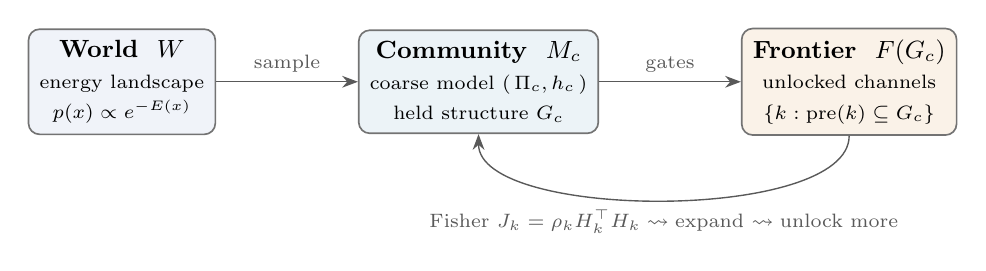
\begin{tikzpicture}[node distance=7mm]
  \node[box,fill=costc!7] (W) {\textbf{World } $W$\\\scriptsize energy landscape\\\scriptsize $p(x)\propto e^{-E(x)}$};
  \node[box,fill=corec!8,right=18mm of W] (M) {\textbf{Community } $M_c$\\\scriptsize coarse model $(\,\Pi_c,h_c\,)$\\\scriptsize held structure $G_c$};
  \node[box,fill=newc!10,right=18mm of M] (F) {\textbf{Frontier } $F(G_c)$\\\scriptsize unlocked channels\\\scriptsize $\{k:\Prereq(k)\subseteq G_c\}$};
  \draw[flow] (W) -- node[above,font=\scriptsize]{sample} (M);
  \draw[flow] (M) -- node[above,font=\scriptsize]{gates} (F);
  \draw[flow] (F.south) .. controls +(0,-1.1) and +(0,-1.1) .. (M.south)
      node[midway,below,font=\scriptsize,align=center]{Fisher $J_k=\rho_k H_k^\top H_k$\;$\rw$\;expand $\rw$\;unlock more};
\end{tikzpicture}
\caption{The environment as three objects and a feedback loop. The world is sampled through whatever
channels the community has unlocked; the resulting information grows the held structure $G_c$; the
grown structure widens the frontier $F(G_c)$. \S\ref{sec:energy}--\ref{sec:frontier} formalize each
box and the loop.}
\label{fig:overview}
\end{figure}

% ======================================================================
\section{The world as an energy landscape}
\label{sec:energy}
% ======================================================================

Read the world thermodynamically. A configuration $x$ has an \emph{energy} $E(x)$ and the world's
law is the Gibbs measure $p(x)=Z^{-1}e^{-E(x)}$, $Z=\int e^{-E(x)}\,dx$
\citep{jaynes1957}. For any strictly positive law the Hammersley--Clifford theorem makes the energy
a sum of clique potentials of an undirected graph $\mathcal G^\ast=(V,\mathcal E^\ast)$,
\begin{equation}
E(x)=\sum_{C\in\mathrm{cl}(\mathcal G^\ast)}\varphi_C(x_C),
\label{eq:hc}
\end{equation}
so the \emph{shape of the energy is the graph}: $x_i\perp x_j\mid x_{\setminus ij}$ exactly when no
clique holds both \citep{besag1974}. The tractable corner we use throughout is the Gaussian (Gauss--
Markov) field, where the potentials are quadratic and
\begin{equation}
E(x)=\tfrac12\,x^\top\Pi^\ast x-h^{\ast\top}x,\qquad
p(x)=\mathcal N\!\big((\Pi^\ast)^{-1}h^\ast,\ (\Pi^\ast)^{-1}\big),
\label{eq:gmrf}
\end{equation}
with the \emph{precision} $\Pi^\ast\succ0$ playing the role of the energy's Hessian; its zero pattern
is $\mathcal G^\ast$. ``Deep substructure'' is then a literal statement about $\Pi^\ast$: order the
fine variables into a dense, high-precision \emph{core}, a layer of \emph{mechanisms}, and a sparse
observable \emph{belt}, and $\Pi^\ast$ is block-structured by depth (Fig.~\ref{fig:energy}, right).
Beyond the Gaussian corner the same energy carries the feature that makes the world hard: many
\emph{metastable basins} organised hierarchically---the ultrametric landscape of spin glasses
\citep{mpv1987}, the associative-memory energy of \citet{hopfield1982}. A basin is a candidate
theory; the barrier between two basins is the energy a learner must pay to move between them---the
cost of revising a commitment (Fig.~\ref{fig:energy}, left). The world is not a target to be guessed
but a landscape to be traversed.

\begin{figure}[h]
\centering
\begin{subfigure}{0.52\textwidth}\centering
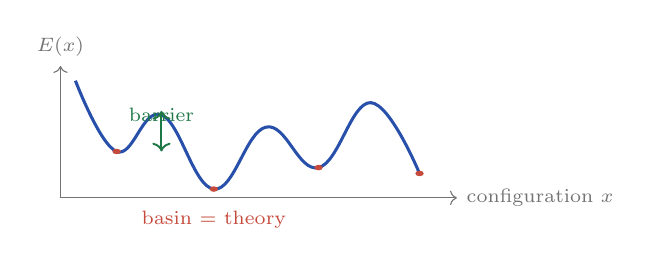
\begin{tikzpicture}[yscale=0.62,xscale=0.95]
  \draw[->,black!55] (-0.2,0)--(5.1,0) node[right,font=\scriptsize]{configuration $x$};
  \draw[->,black!55] (-0.2,0)--(-0.2,2.7) node[above,font=\scriptsize]{$E(x)$};
  \draw[costc,line width=1.1pt,smooth,tension=0.7]
     plot coordinates {(0,2.4)(0.55,0.95)(1.15,1.7)(1.85,0.18)(2.55,1.45)(3.25,0.62)(3.95,1.95)(4.6,0.5)};
  \foreach \p/\lab in {(0.55,0.95)/, (1.85,0.18)/, (3.25,0.62)/, (4.6,0.5)/}
     {\fill[scalarc] \p circle (1.6pt);}
  \node[font=\scriptsize,scalarc] at (1.85,-0.45) {basin = theory};
  \draw[<->,gradc,line width=0.7pt] (1.15,1.78) -- node[above,font=\scriptsize,text=gradc]{barrier} (1.15,0.95);
\end{tikzpicture}
\caption{energy profile: basins and barriers}
\label{sub:basins}
\end{subfigure}
\hfill
\begin{subfigure}{0.44\textwidth}\centering
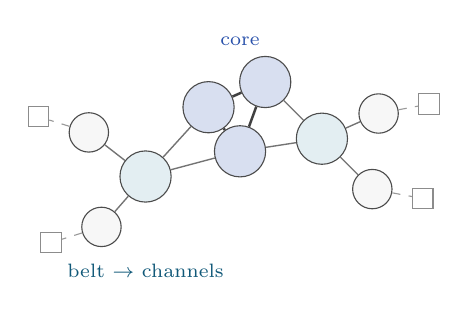
\begin{tikzpicture}[scale=0.8]
  % core
  \node[bel,fill=costc!18] (c1) at (0,1.1){}; \node[bel,fill=costc!18] (c2) at (0.9,1.5){};
  \node[bel,fill=costc!18] (c3) at (0.5,0.4){};
  \draw[core] (c1)--(c2)--(c3)--(c1);
  % mechanisms
  \node[bel,fill=corec!12] (m1) at (-1.0,0.0){}; \node[bel,fill=corec!12] (m2) at (1.8,0.6){};
  \draw[belt] (c1)--(m1); \draw[belt] (c3)--(m1); \draw[belt] (c2)--(m2); \draw[belt] (c3)--(m2);
  % belt + observations
  \foreach \i/\x/\y in {1/-1.9/0.7, 2/-1.7/-0.8, 3/2.7/1.0, 4/2.6/-0.2}{
     \node[bel,minimum size=5mm,fill=black!3] (b\i) at (\x,\y){};}
  \draw[belt] (m1)--(b1); \draw[belt] (m1)--(b2); \draw[belt] (m2)--(b3); \draw[belt] (m2)--(b4);
  \foreach \i/\x/\y in {1/-2.7/0.95, 2/-2.5/-1.05, 3/3.5/1.15, 4/3.4/-0.35}{
     \node[obs] (o\i) at (\x,\y){}; }
  \draw[sens] (b1)--(o1); \draw[sens] (b2)--(o2); \draw[sens] (b3)--(o3); \draw[sens] (b4)--(o4);
  \node[font=\scriptsize,costc] at (0.5,2.15){core};
  \node[font=\scriptsize,corec!80!black] at (-1.0,-1.5){belt $\to$ channels};
\end{tikzpicture}
\caption{the precision graph $\mathcal G^\ast$ of $\Pi^\ast$}
\label{sub:graph}
\end{subfigure}
\caption{The world is an energy landscape. \subref{sub:basins}~In non-Gaussian energies the landscape
is rugged: basins are candidate theories and the barrier between them is the revision cost.
\subref{sub:graph}~The sparsity of the Gaussian precision $\Pi^\ast$ \emph{is} the dependency graph;
depth runs core (dense) $\to$ mechanisms $\to$ belt, and only the belt touches observation channels
(squares).}
\label{fig:energy}
\end{figure}

% ======================================================================
\section{The world as a graphical model, and learning as structure search}
\label{sec:pgm}
% ======================================================================

Read the same world causally. Factor the Gaussian field as a linear structural equation model on a
weighted DAG,
\begin{equation}
x=Ax+\zeta,\quad \zeta\sim\mathcal N(0,D^{-1}),\qquad
\Pi^\ast=(I-A)^\top D\,(I-A),\quad \Top=(I-A)^{-1}=\sum_{k\ge0}A^{k},
\label{eq:sem}
\end{equation}
so $x=\Top\zeta$ and $p(x)=\prod_i p(x_i\mid x_{\mathrm{pa}(i)})$ is the Markov factorization of
\citet{pearl2009,kollerfriedman2009}; $\Top$ is the \emph{propagation operator} that carries a
perturbation at one node to all its descendants. A community is a \emph{belief} over this structure,
held in the same information form, $M_c=(\Pi_c,h_c)$ on a node set $V_c\subseteq V$. The world enters
a belief only through measurement. An \emph{observation channel} $k$ reads a linear combination
$o_k=H_k x+\varepsilon_k$, $\varepsilon_k\sim\mathcal N(0,\rho_k^{-1}I)$, and the conjugate update
adds its Fisher information to the precision,
\begin{equation}
\Pi_c\ \leftarrow\ \Pi_c+\!\!\sum_{k\in F(G_c)}\!\! J_k,\qquad
J_k=\rho_k\,H_k^\top H_k,\qquad j_k=\rho_k\,H_k^\top o_k,
\label{eq:fisher}
\end{equation}
the sum running only over \emph{unlocked} channels $F(G_c)$---the coupling to \S\ref{sec:frontier}.
The Fisher term $J_k$ is also the metric of the statistical manifold on which the belief moves, so
learning is natural-gradient descent on variational free energy \citep{amari2016}.

Learning the \emph{structure}, not just the state, is two moves of asymmetric cost
(Fig.~\ref{fig:pgm}). Each candidate edge $e$ carries an automatic-relevance-determination prior
precision $\alpha_e$, with $\alpha_e\!\to\!\infty$ pinning the edge off and $\alpha_e\!\to\!0$ freeing
it \citep{mackay1992,neal1996,tipping2001}. \emph{Reduction} prunes an edge the data no longer
support; because a reduced model shares its likelihood and differs only in its prior, the change in
evidence is closed form---the Savage--Dickey ratio of Bayesian model reduction,
\begin{equation}
\frac{p(o\mid\tilde M)}{p(o\mid M)}=\Eq{p(\theta\mid o)}{\frac{\tilde p(\theta)}{p(\theta)}},
\qquad \Delta F>0\ \Rightarrow\ \text{prune},
\label{eq:bmr}
\end{equation}
read off the already-inverted posterior \citep{friston2018bmr}. \emph{Expansion} proposes a
commitment not yet represented---bordering a new node $N$ wired at free priors and letting reduction
carve it back \citep{friston2017curiosity}. Expansion is the costly half: a genuinely new node may
open an observable channel and so enlarge the likelihood's support, the one real inversion the cheap
closed form is spared. This is the formal seam at which \S\ref{sec:frontier} cuts---the move that
\emph{unlocks an observation} is exactly model expansion.

\begin{figure}[h]
\centering
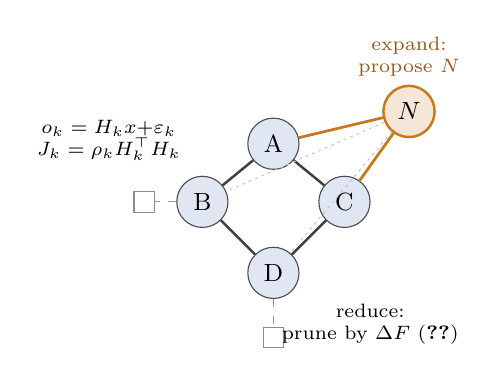
\begin{tikzpicture}[scale=0.82]
  \node[bel,fill=costc!14](A) at (0,1){A}; \node[bel,fill=costc!14](B) at (-1.1,0.1){B};
  \node[bel,fill=costc!14](C) at (1.1,0.1){C}; \node[bel,fill=costc!14](D) at (0,-1){D};
  \draw[core](A)--(B); \draw[core](A)--(C); \draw[core](B)--(D); \draw[core](C)--(D);
  % new node
  \node[bel,draw=newc,line width=0.9pt,fill=newc!18](N) at (2.1,1.5){$N$};
  \draw[newc,line width=1.0pt](N)--(A); \draw[newc,line width=1.0pt](N)--(C); % survivors
  \draw[black!22,dash pattern=on 1pt off 1.5pt](N)--(B); \draw[black!22,dash pattern=on 1pt off 1.5pt](N)--(D);
  \node[font=\scriptsize,newc!75!black,align=center] at (2.1,2.35){expand:\\propose $N$};
  % observation channels depositing Fisher
  \foreach \nd/\x/\y in {B/-2.0/0.1, D/0/-2.0}{
    \node[obs] (o\nd) at (\x,\y){};}
  \draw[sens](B)--(oB); \draw[sens](D)--(oD);
  \node[font=\scriptsize,align=center] at (-2.55,1.05){$o_k=H_kx{+}\varepsilon_k$\\$J_k=\rho_kH_k^\top H_k$};
  \node[font=\scriptsize,align=center] at (1.5,-1.8){reduce:\\prune by $\Delta F$ \eqref{eq:bmr}};
\end{tikzpicture}
\caption{Learning as structure search. Observation channels (squares) deposit Fisher information
\eqref{eq:fisher} into the belief; \emph{expansion} borders a new node $N$ at free priors (amber) and
\emph{reduction} prunes the candidate edges the data do not hold (faint) in closed form
\eqref{eq:bmr}. Expansion is the move that can open a new channel---the hinge to
\S\ref{sec:frontier}.}
\label{fig:pgm}
\end{figure}

% ======================================================================
\section{Coarse-graining: where a community starts}
\label{sec:coarse}
% ======================================================================

A community does not start with $\mathcal G^\ast$; it starts \emph{coarse}. Formalize a coarse model
as a partition $P_c=\{B_1,\dots,B_m\}$ of the fine nodes $V$ into super-nodes, with aggregation map
$S_c\in\{0,1\}^{m\times n}$, $(S_c)_{ai}=1\Leftrightarrow i\in B_a$. The coarse variable is
$y=S_c x$, and integrating out the within-block fluctuation gives the effective (Gaussian) energy
\begin{equation}
e^{-E_c(y)}\ \propto\!\!\int\!\! e^{-E(x)}\,\delta(S_c x-y)\,dx
\quad\Longrightarrow\quad
\Pi_c=\big(S_c\,(\Pi^\ast)^{-1}S_c^\top\big)^{-1},
\label{eq:coarse}
\end{equation}
the block-aggregated precision (the Schur reduction onto the super-nodes; in the repository this is
\texttt{bmr.schur\_marginalize}). Equation~\eqref{eq:coarse} is one blocking step of the
renormalization group: replace fluctuating fine detail by a super-node and read the induced
effective couplings \citep{kadanoff1966,wilson1975,jonalasinio1975}. The coarse model is
\emph{exact}---a faithful lower-resolution copy---only when the partition is strongly lumpable, i.e.\
respects the dependency structure so that block members are interchangeable \citep{kemenysnell1976};
generic partitions are not lumpable, and then a coarse model is strictly weaker: it senses only
aggregates, resolves the world more slowly the coarser it is, and under forgetting plateaus at a
residual it can never clear. Crucially, \textbf{refinement is expansion}: splitting a super-node into
two is the addition of a node (\S\ref{sec:pgm}), a single step \emph{up} the partition lattice
(Fig.~\ref{fig:coarse}). The lattice of partitions, ordered by refinement, is therefore the scaffold
on which the next section's frontier climbs---and where a community sits on it at $t=0$ is its
\emph{seed}.

\begin{figure}[h]
\centering
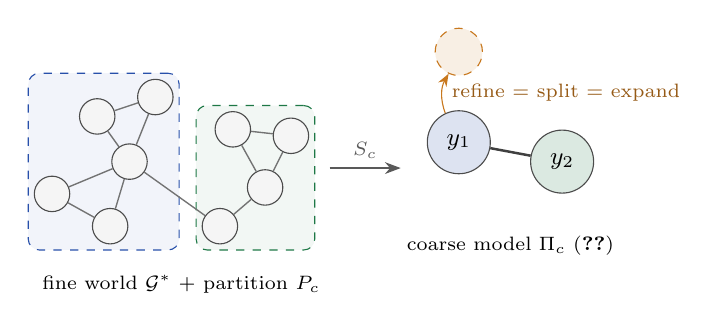
\begin{tikzpicture}[scale=0.82]
  % fine graph (left)
  \begin{scope}[xshift=0cm]
   \foreach \i/\x/\y in {1/0/1.2, 2/0.9/1.5, 3/0.5/0.5, 4/-0.7/0.0, 5/0.2/-0.5,
                         6/2.1/1.0, 7/2.6/0.1, 8/1.9/-0.5, 9/3.0/0.9}{
     \node[bel,minimum size=4.5mm,fill=black!4] (f\i) at (\x,\y){};}
   \draw[belt](f1)--(f2)--(f3)--(f1); \draw[belt](f3)--(f4)--(f5)--(f3);
   \draw[belt](f6)--(f7)--(f8); \draw[belt](f6)--(f9)--(f7); \draw[belt](f3)--(f8);
   \begin{scope}[on background layer]
     \node[draw=costc,dashed,rounded corners,fill=costc!6,fit=(f1)(f2)(f3)(f4)(f5),inner sep=2pt]{};
     \node[draw=gradc,dashed,rounded corners,fill=gradc!6,fit=(f6)(f7)(f8)(f9),inner sep=2pt]{};
   \end{scope}
   \node[font=\scriptsize] at (1.3,-1.4){fine world $\mathcal G^\ast$ + partition $P_c$};
  \end{scope}
  % arrow
  \draw[flow] (3.6,0.4)--node[above,font=\scriptsize]{$S_c$}(4.7,0.4);
  % coarse graph (right)
  \begin{scope}[xshift=5.6cm,yshift=0.2cm]
    \node[bel,minimum size=8mm,fill=costc!16] (Y1) at (0,0.6){$y_1$};
    \node[bel,minimum size=8mm,fill=gradc!16] (Y2) at (1.6,0.3){$y_2$};
    \draw[core](Y1)--(Y2);
    \node[font=\scriptsize] at (0.8,-1.0){coarse model $\Pi_c$ \eqref{eq:coarse}};
    % refine = split
    \node[bel,draw=newc,dashed,minimum size=6mm,fill=newc!12] (sp) at (0.0,2.0){};
    \draw[newc,-{Stealth[length=1.6mm]}] (Y1) to[bend left=25] node[right,font=\scriptsize,text=newc!75!black]{refine = split = expand} (sp);
  \end{scope}
\end{tikzpicture}
\caption{Coarse-graining as a starting structure. A partition $P_c$ of the fine world (left, two
blocks) aggregates by $S_c$ to a coarse model $\Pi_c$ (right) via the renormalization step
\eqref{eq:coarse}. Refining---splitting a super-node---is a model-expansion move, one step up the
partition lattice. A community's seed is where it sits on that lattice at $t=0$.}
\label{fig:coarse}
\end{figure}

% ======================================================================
\section{The endogenous observation frontier}
\label{sec:frontier}
% ======================================================================

Here is the ingredient that makes the environment its own thing. Let $\Omega$ be the ground set of
structural elements (candidate nodes and edges), and let a community's \emph{held structure}
$G\subseteq\Omega$ be the subgraph it currently commits to; its seed $G_c(0)$ is the coarse model of
\S\ref{sec:coarse}. Each channel $k$ carries a \emph{prerequisite} $\Prereq(k)\subseteq\Omega$, and
the world is legible to a community only through the channels its structure has earned.

\begin{definition}[Frontier]
The \emph{unlocked frontier} at held structure $G$ is
$F(G)=\{\,k\in K:\ \Prereq(k)\subseteq G\,\}$. It is monotone: $G\subseteq G'\Rightarrow F(G)\subseteq
F(G')$---more structure never hides a channel.
\end{definition}

\noindent Observing through $F(G)$ deposits the Fisher information \eqref{eq:fisher} of exactly those
channels, and that information is what licenses the next expansion (\S\ref{sec:pgm}): a structural
element $\omega\in\Omega$ becomes \emph{data-supported} only when the channels loading on it are
unlocked. Collect one round of supported growth into an operator.

\begin{definition}[Unlock operator]
$\displaystyle \Phi(G)=G\ \cup\ \big\{\omega\in\Omega:\ \omega\ \text{is data-supported under the
channels}\ F(G)\big\}.$ It is \emph{extensive} ($G\subseteq\Phi(G)$) and \emph{monotone}
($G\subseteq G'\Rightarrow\Phi(G)\subseteq\Phi(G')$), because a wider frontier can only add support.
\end{definition}

A community's trajectory is the orbit $G_c(t{+}1)=\Phi(G_c(t))$ from its seed: structure unlocks
channels, channels supply Fisher, Fisher supports expansion, expansion is more structure
(Fig.~\ref{fig:frontier}\subref{sub:tree}). Because $\Omega$ is finite the orbit is an increasing
chain in $2^\Omega$ and halts.

\begin{proposition}[Seed-determined closure and structural pluralism]
\label{prop:fix}
On the finite lattice $2^\Omega$, $\Phi$ monotone and extensive has, above any seed $G_0$, a unique
least fixed point $G^\star(G_0)=\bigcup_{t\ge0}\Phi^t(G_0)$ \citep[Knaster--Tarski;][]{tarski1955}.
The learned structure is a function of the seed alone. Hence two disconnected communities with seeds
$G_0^A,G_0^B$ for which $G^\star(G_0^A)\neq G^\star(G_0^B)$ end with different unlocked frontiers
$F(G^\star)$: they cannot be brought to the same evidence, because each lacks a channel the other's
theory made visible. Pluralism is the \emph{multiplicity of fixed points of the unlock operator}, not
a tuned exploration term.
\end{proposition}

\noindent The family of structures reachable from a seed---closed under the order in which supported
elements are taken---is an \emph{accessible set system}; when prerequisites compose monotonically it
is an \emph{antimatroid}, the order-theoretic skeleton of a dependency ``tech tree''
\citep{kls1991,daveypriestley2002}, with $\Phi$ its closure operator in the sense of formal concept
analysis \citep{ganterwille1999}. The reading is exactly curriculum learning with an endogenous
curriculum \citep{bengio2009}: what a community can next learn to see is set by what it has already
learned. It is also Stanford's problem of unconceived alternatives made structural---a channel never
unlocked is not disbelieved but \emph{unconceived}, and no amount of the evidence it would carry can
reach the community \citep{stanford2006}. Because the world is a rugged landscape (\S\ref{sec:energy})
with no single best basin for a bounded learner \citep{kauffman1993,wolpertmacready1997}, different
seeds settling in different basins is the generic case, not a pathology.

What couples the communities is the social graph. Let $G_{\mathrm{soc}}$ be a stochastic block model
over communities---\texttt{graphs.community}$(\text{sizes},\text{intra},\text{inter})$ in the
repository---with connectivity measured by the Fiedler value
$\lambda_2=\texttt{algebraic\_connectivity}(G_{\mathrm{soc}})$. Communities that share
data-supported proposals advance $\Phi$ on the \emph{union} of their held structures, merging their
frontiers. Thus $\lambda_2$ is the lever on
Proposition~\ref{prop:fix} (Fig.~\ref{fig:frontier}\subref{sub:sbm}): at $\lambda_2=0$ the blocks are
separate echo chambers and seed-distinct fixed points persist (pluralism preserved); raising
$\lambda_2$ merges frontiers and drives the population toward a common fixed point (consensus, or
shared lock-in). Connection collapses structural divergence; disconnection protects it.

\begin{figure}[h]
\centering
\begin{subfigure}{0.62\textwidth}\centering
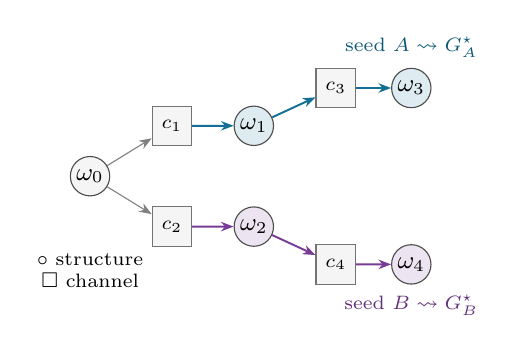
\begin{tikzpicture}[scale=0.8]
  % held-structure circles (omega) and channel squares (c), layered
  \node[bel,minimum size=5mm,fill=black!4] (w0) at (0,0){$\omega_0$};
  \node[ch] (c1) at (1.3,0.8){$c_1$}; \node[ch] (c2) at (1.3,-0.8){$c_2$};
  \node[bel,minimum size=5mm,fill=corec!14] (w1) at (2.6,0.8){$\omega_1$};
  \node[bel,minimum size=5mm,fill=lockc!14] (w2) at (2.6,-0.8){$\omega_2$};
  \node[ch] (c3) at (3.9,1.4){$c_3$}; \node[ch] (c4) at (3.9,-1.4){$c_4$};
  \node[bel,minimum size=5mm,fill=corec!14] (w3) at (5.1,1.4){$\omega_3$};
  \node[bel,minimum size=5mm,fill=lockc!14] (w4) at (5.1,-1.4){$\omega_4$};
  % prereq edges: omega unlocks channel; channel supports omega
  \draw[pre](w0)--(c1); \draw[pre](w0)--(c2);
  \draw[pre,corec,line width=0.7pt](c1)--(w1); \draw[pre,lockc,line width=0.7pt](c2)--(w2);
  \draw[pre,corec,line width=0.7pt](w1)--(c3); \draw[pre,lockc,line width=0.7pt](w2)--(c4);
  \draw[pre,corec,line width=0.7pt](c3)--(w3); \draw[pre,lockc,line width=0.7pt](c4)--(w4);
  \node[font=\scriptsize,corec!80!black] at (5.1,2.05){seed $A\rw G^\star_A$};
  \node[font=\scriptsize,lockc!80!black] at (5.1,-2.05){seed $B\rw G^\star_B$};
  \node[font=\scriptsize,align=center] at (0,-1.5){$\circ$ structure\\$\square$ channel};
\end{tikzpicture}
\caption{the accessible ``tech tree'': two seeds, two fixed points}
\label{sub:tree}
\end{subfigure}
\hfill
\begin{subfigure}{0.34\textwidth}\centering
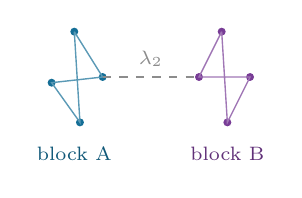
\begin{tikzpicture}[scale=0.72]
  \foreach \i/\x/\y in {1/0/0.9,2/0.5/0.1,3/-0.4/0.0,4/0.1/-0.7}{
     \fill[corec] (\x,\y) circle (2pt);}
  \foreach \i/\x/\y in {1/2.6/0.9,2/2.2/0.1,3/3.1/0.1,4/2.7/-0.7}{
     \fill[lockc] (\x,\y) circle (2pt);}
  \draw[corec!70,line width=0.5pt](0,0.9)--(0.5,0.1)--(-0.4,0.0)--(0.1,-0.7)--(0,0.9);
  \draw[lockc!70,line width=0.5pt](2.6,0.9)--(2.2,0.1)--(3.1,0.1)--(2.7,-0.7)--(2.6,0.9);
  \draw[black!45,dashed,line width=0.6pt](0.5,0.1)--node[above,font=\scriptsize]{$\lambda_2$}(2.2,0.1);
  \node[font=\scriptsize,corec!80!black] at (0.0,-1.25){block A};
  \node[font=\scriptsize,lockc!80!black] at (2.7,-1.25){block B};
\end{tikzpicture}
\caption{social graph $G_{\mathrm{soc}}$ (SBM)}
\label{sub:sbm}
\end{subfigure}
\caption{The endogenous frontier. \subref{sub:tree}~Held structures ($\circ$) unlock channels
($\square$) whose data support the next structure; a seed determines a route and a fixed point, and
two seeds (teal $A$, purple $B$) reach \emph{different} learned structures on the \emph{same} world.
\subref{sub:sbm}~The Fiedler value $\lambda_2$ of the social block model sets whether frontiers stay
separate ($\lambda_2{=}0$, pluralism) or merge ($\lambda_2{>}0$, consensus).}
\label{fig:frontier}
\end{figure}

% ======================================================================
\section{Synthesis: one object, four readings}
\label{sec:synthesis}
% ======================================================================

The four sections are one environment seen from four fields (Table~\ref{tab:dict}). What is true is
an \emph{energy landscape}; how it is represented and learned is a \emph{graphical model under
structure search}; where a community starts is a \emph{coarse-graining}; and what it can come to see
is an \emph{accessible poset} whose fixed points are its possible paradigms. The composition is the
whole claim: a bounded learner, seeded with a coarse model, climbs the partition lattice by expansion
only through the channels its current structure unlocks, and so settles---path-dependently---into one
basin of a landscape that admits many. Nothing in the loop is a free exploration parameter; the
diversity that protects a population is the multiplicity of fixed points, and the one social dial,
$\lambda_2$, decides whether that diversity survives.

\begin{table}[h]
\centering\footnotesize
\renewcommand{\arraystretch}{1.12}
\begin{tabular}{@{}p{0.205\linewidth}p{0.215\linewidth}p{0.235\linewidth}p{0.235\linewidth}@{}}
\hline
\textbf{Reading} & \textbf{Object} & \textbf{Borrowed from} & \textbf{Closed form / handle}\\
\hline
Energy landscape & world law $p(x)\propto e^{-E(x)}$ & Gibbs / spin glass \citep{hopfield1982,mpv1987} & $\Pi^\ast$ = energy Hessian \eqref{eq:gmrf}\\
Graphical model & belief $(\Pi_c,h_c)$, learning & PGM + active inference \citep{pearl2009,friston2018bmr} & Fisher $J_k$, BMR $\Delta F$ \eqref{eq:fisher},\eqref{eq:bmr}\\
Coarse-graining & seed $P_c$, super-nodes & RG / lumpability \citep{wilson1975,kemenysnell1976} & $\Pi_c=(S_c\Sigma^\ast S_c^\top)^{-1}$ \eqref{eq:coarse}\\
Accessible poset & frontier $F$, closure $\Phi$ & order theory \citep{kls1991,tarski1955} & least fixed point $G^\star$ (Prop.~\ref{prop:fix})\\
\hline
\end{tabular}
\caption{The dictionary. Each row is the same environment under a different field's first principles;
the right column is the quantity that makes the reading computable.}
\label{tab:dict}
\end{table}

% ======================================================================
\begin{thebibliography}{99}\footnotesize\setlength{\itemsep}{0.5pt}\setlength{\parskip}{0pt}
% ======================================================================
\bibitem[Amari(2016)]{amari2016} Amari, S. (2016). \emph{Information Geometry and Its Applications}. Springer.
\bibitem[Bengio et al.(2009)]{bengio2009} Bengio, Y., Louradour, J., Collobert, R., \& Weston, J. (2009). Curriculum learning. \emph{ICML}, 41--48.
\bibitem[Besag(1974)]{besag1974} Besag, J. (1974). Spatial interaction and the statistical analysis of lattice systems. \emph{J. R. Stat. Soc. B}, 36(2), 192--236.
\bibitem[Davey \& Priestley(2002)]{daveypriestley2002} Davey, B. A., \& Priestley, H. A. (2002). \emph{Introduction to Lattices and Order} (2nd ed.). Cambridge University Press.
\bibitem[Friston et al.(2017)]{friston2017curiosity} Friston, K., Lin, M., Frith, C. D., Pezzulo, G., Hobson, J. A., \& Ondobaka, S. (2017). Active inference, curiosity and insight. \emph{Neural Computation}, 29(10), 2633--2683.
\bibitem[Friston et al.(2018)]{friston2018bmr} Friston, K., Parr, T., \& Zeidman, P. (2018). Bayesian model reduction. \emph{arXiv:1805.07092}.
\bibitem[Ganter \& Wille(1999)]{ganterwille1999} Ganter, B., \& Wille, R. (1999). \emph{Formal Concept Analysis: Mathematical Foundations}. Springer.
\bibitem[Hopfield(1982)]{hopfield1982} Hopfield, J. J. (1982). Neural networks and physical systems with emergent collective computational abilities. \emph{PNAS}, 79(8), 2554--2558.
\bibitem[Jaynes(1957)]{jaynes1957} Jaynes, E. T. (1957). Information theory and statistical mechanics. \emph{Physical Review}, 106(4), 620--630.
\bibitem[Jona-Lasinio(1975)]{jonalasinio1975} Jona-Lasinio, G. (1975). The renormalization group: A probabilistic view. \emph{Il Nuovo Cimento B}, 26(1), 99--119.
\bibitem[Kadanoff(1966)]{kadanoff1966} Kadanoff, L. P. (1966). Scaling laws for Ising models near $T_c$. \emph{Physics}, 2(6), 263--272.
\bibitem[Kauffman(1993)]{kauffman1993} Kauffman, S. A. (1993). \emph{The Origins of Order: Self-Organization and Selection in Evolution}. Oxford University Press.
\bibitem[Kemeny \& Snell(1976)]{kemenysnell1976} Kemeny, J. G., \& Snell, J. L. (1976). \emph{Finite Markov Chains}. Springer.
\bibitem[Koller \& Friedman(2009)]{kollerfriedman2009} Koller, D., \& Friedman, N. (2009). \emph{Probabilistic Graphical Models: Principles and Techniques}. MIT Press.
\bibitem[Korte et al.(1991)]{kls1991} Korte, B., Lov\'asz, L., \& Schrijver, A. (1991). \emph{Greedoids}. Springer.
\bibitem[MacKay(1992)]{mackay1992} MacKay, D. J. C. (1992). Bayesian interpolation. \emph{Neural Computation}, 4(3), 415--447.
\bibitem[M\'ezard et al.(1987)]{mpv1987} M\'ezard, M., Parisi, G., \& Virasoro, M. A. (1987). \emph{Spin Glass Theory and Beyond}. World Scientific.
\bibitem[Neal(1996)]{neal1996} Neal, R. M. (1996). \emph{Bayesian Learning for Neural Networks}. Springer.
\bibitem[Pearl(2009)]{pearl2009} Pearl, J. (2009). \emph{Causality: Models, Reasoning, and Inference} (2nd ed.). Cambridge University Press.
\bibitem[Stanford(2006)]{stanford2006} Stanford, P. K. (2006). \emph{Exceeding Our Grasp: Science, History, and the Problem of Unconceived Alternatives}. Oxford University Press.
\bibitem[Tarski(1955)]{tarski1955} Tarski, A. (1955). A lattice-theoretical fixpoint theorem and its applications. \emph{Pacific J. Math.}, 5(2), 285--309.
\bibitem[Tipping(2001)]{tipping2001} Tipping, M. E. (2001). Sparse Bayesian learning and the relevance vector machine. \emph{JMLR}, 1, 211--244.
\bibitem[Wilson(1975)]{wilson1975} Wilson, K. G. (1975). The renormalization group: Critical phenomena and the Kondo problem. \emph{Rev. Mod. Phys.}, 47(4), 773--840.
\bibitem[Wolpert \& Macready(1997)]{wolpertmacready1997} Wolpert, D. H., \& Macready, W. G. (1997). No free lunch theorems for optimization. \emph{IEEE Trans. Evol. Comput.}, 1(1), 67--82.
\end{thebibliography}

\end{document}
